%version of 03-07-19

\chapter{NUMBERS III: ON NUMBER REPRESENTATIONS}
\label{ch:numerals}

\section{Introduction}

Numbers are intangible idealizations.  One must endow numbers with
names before one can manipulate them and compute with them.
Historically, we have employed a broad range of mechanisms for naming
numbers.

{\ignore {\Arny I really like the idea of providing some cultural
    background to get the reader involved.}}
{\ignore {\Denis I also like the idea, may be we can shorten the Latin numbers
  and let some parts (examples) as an exercice...}}
{\ignore {\Arny Please propose what to omit.  I do want to point out the
  ``three levels'' of names/numerals: names that convey information
  only by cultural agreement; names that permit identification but no
  practical manipulation; {\em operational} names}}
\ignore{I am not sure, however, how much space to
  allocate.  For instance, I like the mention of Roman numerals and of
  the system that the Phoenicians used --- which I am familiar with
  mainly because of Hebrew --- but I am reluctant to go so far as to
  really discuss the formation rules of Roman numerals or the details
  of numeral formation in Hebrew and its kindred languages.}

\medskip

\noindent
{\it Nicknames for ``familiar'' numbers}.
%
We have endowed several numbers that are associated with concrete
entities (see the examples below) with names that do not even hint at
any aspect of the nature of the named number.  A few examples:
\begin{itemize}
\item
$\pi$: the ratio of the circumference of a circle to its diameter
\item
$e$: the base of so-called natural logarithms
\item
$\phi$: the {\it golden ratio} (one of several word-names for $\phi$)
  that can be observed in nature, e.g., in the leaf patterns of plants
  such as pineapples and cauliflower
\item
Avogadro's number: a fundamental quantity in chemistry and physics.
(This number-name indicates that not all numerical nicknames are
single letters.)
\end{itemize}
Nickname-based numerals give no information about the named number:
they do not help anyone (except the {\it cognoscenti:} the
``in-crowd'') {\em identify} the named number, and they do not help
anyone manipulate---e.g., compute with---it.  These names are valuable
only for {\em cultural} purposes, not mathematical ones.

To clarify our intended message: It is the {\em names} of these
special numbers that convey no operational information.  Each of these
is attached to valuable science and/or mathematics!  We shall expose
some of this mathematics as we discuss $e$ in the current chapter,
revisit $\pi$ and $e$ in Chapter~\ref{ch:Summation}, and revisit
$\phi$ in Chapter~\ref{ch:Recurrences}.

\medskip

\noindent
{\it Alphabet-based systems.}
%
Several cultures have developed systems for naming arbitrary integers
by using their alphabets in some manner.  One such system that is
still visible in European cultures comprises {\it Roman
  numerals}. \index{numerals!Roman} One stills encounters these within
constrained contexts, e.g., as the hour markers on the faces of
``classical'' clocks and as timestamps on the cornerstones of official
buildings.  Roman numerals are formed from a constrained set of
letters from the Latin alphabet:

\begin{tabular}{c|c}
{\it Letter} & {\it Numerical value} \\
\hline
I  & 1 \\
V  & 5 \\
X  & 10 \\
L  & 50 \\
C  & 100 \\
D  & 500 \\
M  & 1000
\end{tabular}

\noindent
The formation rules for Roman numerals of length exceeding $2$ are a
bit complicated, but {\em roughly}, a letter to the right of a higher
valued letter augments the value of the numeral (e.g., DCL $=650$, XVI
$=16$), while a letter to the left of a higher valued letter lowers
the value (e.g., MCM $=1900$, XLIV $=44$).

Yet another way to craft numerals from letters is observable in the
based on, e.g., the Hebrew alphabet; \index{numerals!Hebrew} this
system assimilates ideas used by the ancient Egyptians, Phoenicians,
and Greeks.  Hebrew assigns the following respective values to the
$22$ letters of its alphabet.
\[ 1, 2, 3, 4, 5, 6, 7, 8, 9, 10,
20, 30, 40, 50, 60, 70, 80, 90, 100,
 200, 300, 400
\]
Numerals are then formed as strings of single occurrences of letters,
by accumulating the letters' numerical values.  Numbers that are too
large to be named using strings of single letter-instances often allow
repeated letter instances or incorporate auxiliary words, in a
mixed-mode manner similar to our writing the number $5000$ as ``$5$
thousand''.  

{\ignore {\Denis I am not familiar with Hebrew, I would like to know
    how to address the unicity of the writing numbers...}}  {\ignore
{\Arny I am familiar with Hebrew numerals in only two contexts:

(a) They are used widely with the (Hebrew) calendar.  The names of the
  Hebrew months are Babylonian in origin.  The days are always
  denoted by Hebraic numerals.  Within a religious framework, there is
  a number that is associated with the age of the world (since
  ``creation'').  This number was computed by a Catholic monk many
  centuries ago, based on his reading of the Old Testament.  The Jews
  have adopted this number --- and they usually express it with a
  ``mixed'' Hebraic numeral of the form ``5 thousands plus abcd''.  In
  a semi-religious context such as a gravestone, e.g., all of the
  relevant numerals are denoted by Hebraic numerals.

(b) They are used widely as part of a semi-mystical exercise called
  ``gematria''.  Since every numeral is potentially a word, certain
  numbers gain semi-mystical importance.  The mystics use this a lot
  in interpreting biblical texts.  Perhaps the most POPULAR instance
  of gematria relates to the Hebrew word for ``life'': this two-letter
  word is ``chai''.  It has the numerical value 18.  Even nonreligious
  Jews will acknowledge this by, e.g., giving gifts that are integer
  multiples of 18.  For instance, a gift in the amount of 50 dollars is
  usually ``rounded up'' to 54.

I BELIEVE that the numerals were once used more widely, but I know
little about that.}}

Alphabet-based systems for creating numerals are more useful than
nickname-based systems: they {\em do} allow anyone to {\em identify}
any named number. Indeed, one can (algorithmically) convert any Roman
numeral or any Hebrew numeral to a decimal numeral for the same
number.  However, any reader who is familiar with alphabet-based
systems will recognize a major drawback of such systems: It is {\em
  exceedingly difficult} to do any but the most trivial arithmetic
using such systems' numerals.  Two simple examples using Roman
numerals will make our case:
\begin{itemize}
\item
Square CC.  This is, of course, trivial using our familiar decimal
numerals: an elementary school student can compute $200 \times 200 \ =
\ 40,000$.  But even in an early course on programming, one would not
assign the general ``multiply numbers using Roman numerals'' problem
as a first assignment.

\item
Substract MCMXCVIII from MMII.  We all know, of course, that the answer
is IV, but determining this is usually done by converting to decimal numerals
($2002-1998$).
\end{itemize}

\noindent
{\it Positional number systems.}
%
In our daily commerce, we typically deal with numerals that are formed
within a {\it base-$b$ positional number system,}
\index{numerals in a (base-$b$) positional number system}
%
i.e., by strings of {\it digits} from a set of the form $\{0, 1, 2,
\ldots, \overline{b-1}\}$, often embellished with other symbols, such as
a {\em radix point},\footnote{The use of a period as the radix point
  is a US convention; in much of Europe, a comma usually denotes the
  radix point.}~and sometimes a leading ``$+$'' or ``$-$'' to
indicate, respectively, the denoted number's positivity or negativity.
\medskip

\noindent \fbox{
\begin{minipage}{0.97\textwidth}
We employ the notation ``$\overline{b-1}$'' to remind ourselves that
in this context ``$b-1$'' is a digit~\index{digit}, not a string; for instance, when
$b = 10$ (the common {\em decimal} base), $\overline{b-1}$ is the
digit $9$.

\end{minipage}
}

\medskip

\noindent
We discuss positional number systems in detail in the remainder of
this chapter.  For now, we settle for a few examples:
\begin{itemize}
\item
Most of our daily work employs the base-$10$ ({\it decimal}) system,
whose digits comprise the set $\{0, 1, 2, 3, 4, 5., 6, 7, 8, 9\}$; the
system's radix point is usually called a {\em decimal point}.

\item
Because electrical and electronic circuitry are (for the most part)
built using {\it bistable} devices---e.g., switches that are either
{\em on} or {\em off}---the system most often employed when dealing
with such circuitry and its end products (say, computers) is the
base-$2$ ({\it binary}) system, whose digits---usually called {\it
  bits}---comprise the set $\{0, 1\}$.
  The term bit is the contraction of binary digit. 

\item
Because of its small repertoire of digits, the binary system's
numerals are quite long---roughly $3$ times longer than decimal
numerals.  For instance,
\[ 32,768 \ \mbox{ base $10$} \ \ = \ 1,000,000,000,000,000 \ \mbox{
  base $2$}
\]
In order to make these numerals easier for humans to deal with, small
sequences of bits are often aggregated to form larger number bases---but
still powers of $2$.  Two aggregations have been particularly popular:
  \begin{itemize}
  \item
By aggregating length-$3$ sequences of bits, one converts binary
numerals to base-$8$ ({\it octal}) numerals; the octal digits comprise
the set $\{0, 1, 2, 3, 4, 5, 6, 7\}$.
  \item
By aggregating length-$4$ sequences of bits, one converts binary
numerals to base-$16$ ({\it hexadecimal}) numerals; the hexadecimal
digits comprise the set
\[ \{0, 1, 2, 3, 4, 5, 6, 7, 8, 9, \overline{10}, \overline{11},
\overline{12}, \overline{13}, \overline{14}, \overline{15}\}.
\]
{\it Note:} We have written the hexadecimal digits in decimal, to make
them easy to read, but we have placed overlines above the $2$-digit
(decimal) numerals ``$10$'', ``$11$'', ``$12$'', ``$13$'', ``$14$'',
and ``$15$'' as a reminder that each represents a single hexadecimal
digit, not a $2$-digit numeral.
  \end{itemize}
\end{itemize}


\section{Numerals We Can Work With}\index{numerals}
\label{sec:Numerals}


\subsection{Positional Number Systems}
\label{sec:positional-numbers}
\index{positional number system}

The most common family of {\em operational}
\index{numerals!operational} numerals for real numbers---i.e.,
numerals that enable one to do things such as perform arithmetic (add,
multiply, etc.) on the named numbers---is the family of {\it
  positional number systems}.  Each system in this family is
identified by its {\em base}, 
\index{positional number system!base}
which is usually\footnote{In rather specialized contexts one
  encounters number bases that are not positive integers.}~an
integer $b >1$.
\index{positional number system!base-$b$ numeral}
For any base $b$, we define the set $B_b = \{ 0, 1, \ldots, b-1\}$ of
{\it digits in base $b$}.\index{positional number system!digits in
  base $b$}
%
To aid legibility, {\em within the context of base-$b$ positional
  numerals}, we denote the digit $b-1$ as a single character, $\bar{b}$.
\index{$\bar{b}$: the digit $b-1$ in base $b$}
%
We then form base-$b$ numerals in the following way.
\index{positional number system!base-$b$ numerals}
\medskip

\noindent \fbox{
\begin{minipage}{0.97\textwidth}
%\[ \approx \approx \approx \approx \approx \approx \approx \approx \approx \approx \]
{\em The entire edifice of positional numerals builds on the concept
  of {\em geometric summations}, a mathematical structure that we
  shall learn to manipulate, evaluate, and compute with in
  Section~\ref{sec:geometric-sums}.  We need only special aspents of
  this topic here.
}
%\[ \approx \approx \approx \approx \approx \approx \approx \approx \approx \approx \]
\end{minipage}
}
\medskip

{\Denis the following should be put before in 4.5.2}

A base-$b$ numeral is a string having three segments.
\begin{enumerate}
\item
The numeral begins with its {\em integer part},
\index{positional number system!integer part of a numeral}
%
which is a {\em finite} string of digits from $B_b$.  We denote the
integer-part string as: $\alpha_n \alpha_{n-1} \cdots \alpha_1
\alpha_0$.

\item
The numeral continues with a single occurrence of the {\it
  radix point}\index{positional number system!radix point ``$.$''}
``$.$''

\item
The numeral ends with its {\em fractional part},\index{positional
  number system!fractional part of a numeral}
%
which is a string---{\em finite or infinite}--- of digits from $B_b$.
We denote the fractional-part string as:
$\beta_0 \beta_1 \beta_2 \cdots$.
\end{enumerate}
Our completed numeral now has the form
\begin{equation}
\label{eq:real-numeral}
\alpha_n \alpha_{n-1} \cdots \alpha_1 \alpha_0
\ . \ \beta_0 \beta_1 \beta_2 \cdots
\end{equation}
where the $\alpha_i$ and the $\beta_j$
\index{positional number system!base-$b$ digits} 
are {\em base-$b$ digits} i.e., elements of the set $B_b$, and
``$.$'' represents the {\em (base-$b$) radix point}.

\noindent
The numeral depicted in (\ref{eq:real-numeral}) represents the (real)
number\footnote{The notation ``$\mbox{\sc num}_{10}(x)$'' in
  (\ref{eq:real-numeral-number}) denotes an operator that produces the
  {\em numerical value} of the numeral $x$ written in base-$b$.}
\begin{equation}
\label{eq:real-numeral-number}
\mbox{\sc num}_{10}(\alpha_n \alpha_{n-1} \cdots \alpha_1 \alpha_0                  
\ . \ \beta_0 \beta_1 \beta_2 \cdots)
\ \ \eqdef \ \
\sum_{i=0}^n \alpha_i \cdot b^i
\ + \ \sum_{j\geq 0} \beta_j \cdot b^{-j}.
\end{equation}
\index{positional number system!numerical value of numeral}

For emphasis, we note that the base-$b$ integer 
\index{positional number system!numerical value of integral part}
represented by the numeral's integer part is
\[
\mbox{\sc num}_{10}(\alpha_n \alpha_{n-1}\cdots \alpha_1 \alpha_0)
\ \ = \ \
\sum_{i=0}^n \alpha_i \cdot b^i
\]
and the base-$b$ fraction represented by the numeral's fractional part
is\index{positional number system!numerical value of fractional part}
\[
\mbox{\sc num}_{10}(. \beta_0 \beta_1 \beta_2 \cdots)
\ \ = \ \
\sum_{j\geq 0} \beta_j \cdot b^{-j}
\]
By prepending a ``minus sign'' (or, ``negative sign'') $-$ to a
numeral or a number, one renders the thus-embellished entity as
negative.

\medskip

Note that {\em two types of sequences of $0$s do not affect the value
  of the number represented by a numeral:} (1) an {\em initial}
sequence of $0$s to the {\em left} of the radix point and of all
non-$0$ digits; (2) a {\em terminal} sequence of $0$s to the {\em
  right} of the radix point and of all non-$0$ digits.

One consequence of this fact is that we lose no generality by
insisting that every numeral have the following {\em normal form:}
\index{positional number system!numeral!normal form}
\index{normal form for for numeral in a positional number system}

\smallskip

\hspace*{.15in}
\begin{tabular}{l}
-- a finite sequence of digits, \\
-- followed by a radix point, \\
-- followed by an infinite sequence of digits
\end{tabular}


\subsection{Recognizing Integers and  Rationals from Their Numerals}
\label{sec:special-numerals-N-Q}

We have provided an adequate, albeit inelegant, characterization of
the real numbers: a number $r$ is real if, and only if, it can be
represented by an infinite-length numeral in a positional number
system.  Because every rational number---hence, also, every
integer---is also a real number, every rational number and every
integer can also be written as a $b$-ary numeral, in the form
(\ref{eq:real-numeral}).  For rational numbers and integers, we can
make much stronger statements about the forms of their positional
numerals.

{\Denis We have to add a brief discussion about k-ary and k-adic systems...}

\subsubsection{Positional numerals for integers}
\label{sec:special-numerals-N}

\begin{prop}
\label{thm:integer-real}
A real number is an integer if, and only if, it can be represented by
a {\em finite-length} numeral all of whose nonzero digits are to the
left of the radix point.
\index{number!integer!real with a finite numeral}
\end{prop}

\begin{proof}
The result is immediate by definition (\ref{eq:real-numeral-number}).
In the indicated form, if any $\beta_i$ is nonzero, then the {\sc
value} of the numeral is non-integral: it has a nonzero fractional part.
\qed
\end{proof}

We can go beyond the simple statement of
Proposition~\ref{thm:integer-real} and present the following algorithm
that computes the normal-form base-$b$ numeral for an integer $n$.

{\Denis I think it would be better to give the process in literal form as the rest of the chapter...}
\bigskip

\noindent {\underline{\bf Procedure}} {\small\sf Normal-Form
  Numeral}($n$)

/*Compute the normal-form numeral for a given integer $n$*/
\smallskip

\noindent{\bf Initialization}.

Set {\sc current-residue} to $n$
\smallskip

\noindent{\bf Iterate until}
{\sc current-residue} $= 1$

Divide {\sc current-residue} by $b$
\medskip

\noindent
The {\em remainder} upon each division is the next lowest-order
digit in the base-$b$ numeral for $n$.
\bigskip

\noindent {\it Validating the procedure.}
%
The procedure is an implementation of a method of rewriting univariate
polynomials, known variously as {\it Horner's rule} or {\it Horner's
  scheme} \cite{Horner}.  
\index{Horner's rule} \index{Horner's scheme}
Among its other virtues, the ``rule'' provides a recipe for computing
a degree-$d$ univariate polynomial using $O(d)$ multiplications,
rather than the $\Theta(d^2)$ multiplications that appear at first to
be needed.

\medskip

\begin{itemize}
\item {\small\sf The ``standard'' way of writing the polynomial $P(x)$.}

\noindent General degree $d$:

$P(x) \ \ = \ \ a_0 \ + \ a_1 x \ + \ a_2 x^2 \ + \cdots + \ a_{d-1}
x^{d-1} \ + \ a_d x^d$

\noindent Degree $3$:

$P(x) \ \ = \ \ a_0 \ + \ a_1 x \ + \ a_2 x^2 \ + \ a_3 x^3$

\item {\small\sf Rewriting $P(x)$ using Horner's rule.}

\noindent General degree $d$:

$P(x) \ \ = \ \ a_0 \ + \ x \cdot (a_1 \ + \ x \cdot (a_2  \ +  \cdots
+ x \cdot (a_{d-2} \ + \ x \cdot (a_{d-1} \ + \ a_d x)) \cdots ))$  

\noindent Degree $3$:

$P(x) \ \ = \ \ a_0 \ + \ x \cdot (a_1 \ + \ x \cdot (a_2  \ + \ a_3 x))$ 
\end{itemize}

The ``rule'' is so natural that its origins certainly predate the
cited 1819 publication, but they are impossible to trace definitively.  \qed 

\bigskip

\noindent {\it Illustrating the procedure.}
We use the procedure to produce the normal-form base-$2$ (binary)
numeral for $n = 143$.

\medskip

\begin{tabular}{|c|r|r|}
\hline
Step &
{\sc current-residue} &
Remainder \\
\hline
1. & $143$ & $1$ \\
2. & $71$  & $1$ \\
3. & $35$  & $1$ \\
4. & $17$  & $1$ \\
5. & $8$   & $0$ \\
6. & $4$   & $0$ \\
7. & $2$   & $0$ \\
8. & $1$   & $1$ \\
\hline
\end{tabular}

\medskip

\noindent
We have thus derived the following equation which specifies the
base-$2$ normal-form numeral for $143$.
\[ 143_{10} \ = \ 10001111_2 \]


\subsubsection{Positional numerals for rationals}
\label{sec:special-numerals-Q}

We can completely characterize the positional numerals that represent
rational numbers, in terms of the auxiliary notion of an {\em ultimately
  periodic} infinite sequence of digits.
\index{ultimately periodic sequence}

An infinite sequence $S$ of numbers is {\em ultimately periodic} if
there exist two {\em finite} sequences of numbers, $A$ and $B$, such
that $S$ can be written in the following form (we have added spaces to
enhance legibility):
\begin{equation}
\label{eq:ult-per-seq}
 S \ = \ A \ B \ B \ B \cdots B \ B \cdots
\end{equation}
The intention here is that the sequence $B$ is repeated {\it ad
  infinitum}.


\begin{prop}
\label{thm:rational-real}
A positional numeral denotes a rational number if, and only if, it is
ultimately periodic.
\end{prop}

\begin{proof}

\begin{enumerate}
\item 
{\small\sf Part 1: the ``if'' clause.}

Say first that the real number $r$ has an ultimately periodic infinite
base-$b$ numeral.

Since the exact lengths of the finite sequences $A$ and $B$ that
constitute the numeral, as in (\ref{eq:ult-per-seq}), are not germane
to the argument, we arbitrarily denote $r$ by the following
normal-form numeral (spaces added to enhance legibility):
\[  a_2 a_1 a_0 \ . \ b_0 b_1 \
c_0 c_1 c_2 \
c_0 c_1 c_2
\cdots
c_0 c_1 c_2
\cdots
\]
so that
\begin{eqnarray*}
A & = & a_2 a_1 a_0 \ . \ b_0 b_1 \\
B & = & c_0 c_1 c_2
\end{eqnarray*}
(Choosing specific lengths for $A$ and $B$ cuts down on the number of
``ellipsis dots'' we need to denote the numeral, as in ``$123 123
\cdots 123 \cdots$'', hence enhances legibility.)

If we now invoke the evaluation rules of (\ref{eq:real-numeral-number}),
we find that
\begin{eqnarray}
\nonumber
r & = &
\mbox{\sc value}(a_2 a_1 a_0 \ . \ b_0 b_1 \
c_0 c_1 c_2 \
c_0 c_1 c_2
\cdots
c_0 c_1 c_2
\cdots) \\
\nonumber
  & = &
\mbox{\sc value}(a_2 a_1 a_0)
 \ + \ \mbox{\sc value}(b_0 b_1) \cdot b^{-2}
 \ + \
\mbox{\sc value}(c_0 c_1 c_2) \cdot b^{-5} \\
\label{eq:sum-in-numeral}
  &  &
 \ + \
\mbox{\sc value}(c_0 c_1 c_2) \cdot b^{-8}
 \ + \
\mbox{\sc value}(\gamma_0 \gamma_1 \gamma_2) \cdot b^{-11}
\ + \cdots \\
\nonumber
  & = &
\mbox{\sc value}(a_2 a_1 a_0)
 \ + \ \mbox{\sc value}(b_0 b_1) \cdot b^{-2}
 \ + \
\mbox{\sc value}(c_0 c_1 c_2) \cdot \sum_{i=1}^\infty b^{-2-3i}
\end{eqnarray}

{\Denis We must change VALUE, is corresponds to $NUM_{10}$ right?}

We shall learn in Section~\ref{sec:geometric-sums} that infinite
summations such as the one in (\ref{eq:sum-in-numeral}), namely,
$\sum_{i=1}^\infty b^{-2-3i}$,
{\em converge}---meaning that {\em they have finite rational
  sums}---and we learn how to compute these sums.  For the purposes of
the current proof, we just take this fact on faith, and we denote the
summation's finite rational sum by $p/q$.

Collecting all of this information, we find that there exist {\em
  integers} $m$, $n$, $p$, and $q$ such that
\[ r \ = \ m \ + \ n/ b^{2} \ + \ p/q \ = \
\frac{mqb^2 + nq + p}{qb^2}. \]
The number $r$ is, thus, the ratio of two integers; hence, by
definition, it is rational.

\item 
{\small\sf Part 2: the `` only if'' clause.}

Say next that the real number $r$ is rational---specifically,
\[ r \ = \ s + \frac{t}{q} \]
for nonnegative integers $t < q$ and $s$.  It is only the fraction
$t/q < 1$ that can produce an infinite numeral, so it suffices for us
to verify the special case
\[ r \ = \ \frac{t}{q} \ < \ 1 \]
of the proposition.

We prove that $r = t/q$ has an ultimately periodic infinite numeral by
using \index{synthetic division} {\it synthetic division}---the
algorithm taught in elementary school---to compute the ratio $t/q$.
As we proceed, keep in mind that we are working in base $b$.  Each of
the following successive divisions produces one digit to the right of
the radix point, in addition to a possible {\it remainder} $r_i$ from
the set $\{0, 1, \ldots, q-1\}$.
\begin{equation}
\label{eq:build-rational-numeral}
\begin{array}{lclc|l|cc}
\multicolumn{3}{c}{\mbox{Division step}} & &  \hspace*{.15in} \mbox{Current numeral} & &
\mbox{Current remainder} \\
\hline
b \cdot t   & = & a_0 \cdot q \ + \ r_0 &
      & t/q \ = \ .a_0 \cdots &
      & r_0 < q \\
b \cdot r_0 & = & a_1 \cdot q \ + \ r_1 &
      & t/q \ = \ .a_0 a_1 \cdots &
      & r_1 < q \\
            & \vdots &  & & \hspace*{.3in} \vdots &  & \vdots \\
b \cdot r_i & = & a_{i+1} \cdot q \ + \ r_{i+1} &
      & t/q \ = \ .a_0 a_1 \cdots a_{i+1} \cdots &
      & r_{i+1} < q \\
b \cdot r_{i+1} & = & a_{i+2} \cdot q \ + \ r_{i+2} &
      & t/q \ = \ .a_0 a_1 \cdots a_{i+1} a_{i+2} \cdots &
      & r_{i+2} < q \\
            & \vdots &  & &  \hspace*{.3in}\vdots & & \vdots   \\
\end{array}
\end{equation}
Because of the possible values the remainders $r_j$ can assume, no
more than $q$ of the divisions in the (infinite) system
(\ref{eq:build-rational-numeral}) are distinct.  ({\em This is an
  application of the pigeonhole principle
  (Section~\ref{sec:pigeonhole}).})  Because of the way the system
proceeds, once we have encountered two remainders, say, $r_i$ and
$r_{i+k}$, that are equal---i.e., $r_i = r_{i+k}$---we must
thenceforth observe periodic behavior:
\[
\begin{array}{cccccccc}
r_i       & = & r_{i+k}    & = & r_{i+2k}   & = & r_{i+3k}   & = \ \cdots \\
r_{i+1}   & = & r_{i+k+1}  & = & r_{i+2k+1} & = & r_{i+3k+1} & = \ \cdots \\
\vdots    &   & \vdots     &   & \vdots     &   & \vdots     & \\
r_{i+k-1} & = & r_{i+2k-1} & = & r_{i+3k-1} & = & r_{i+4k-1} & = \ \cdots \\
\end{array}
\]
This will engender periodicity in the digits of $r$'s base-$b$ numeral:
\[ [\mbox{\sc initial segment}]
 [a_i a_{i+1} \cdots a_{i+k-1}]
          [a_i a_{i+1} \cdots a_{i+k-1}]
    \cdots  [a_i a_{i+1} \cdots a_{i+k-1}] \cdots 
\]
We are, thus, observing the claimed ultimately periodic behavior in
$r$'s base-$b$ numeral.
\end{enumerate}
\qed
\end{proof}

\bigskip

We end this section by illustrating the process of generating numerals
for rationals via synthetic division.  We employ the fraction $t/q = 4/7$
and base $b = 10$.
\[
\begin{array}{lclc|l|cc}
\multicolumn{3}{c}{\mbox{Division step}} & &  \hspace*{.15in} \mbox{Current numeral} & &
\mbox{Current remainder} \\
\hline
10 \cdot 4   & = & 5 \cdot 7 \ + \ 5 &
      & 4/7 \ = \ .5 \cdots &
      & 5 \\
10 \cdot 5 & = & 7 \cdot 7 \ + \ 1 &
      & 4/7 \ = \ .57 \cdots &
      & 1 \\
10 \cdot 1 & = & 1 \cdot 7 \ + \ 3 &
      & 4/7 \ = \ .571 \cdots &
      & 3 \\
10 \cdot 3 & = & 4 \cdot 7 \ + \ 2 &
      & 4/7 \ = \ .5714 \cdots &
      & 2 \\
10 \cdot 2 & = & 2 \cdot 7 \ + \ 6 &
      & 4/7 \ = \ .57142 \cdots &
      & 6 \\
10 \cdot 6 & = & 8 \cdot 7 \ + \ 4 &
      & 4/7 \ = \ .571428 \cdots &
      & 4 \\
 & \vdots & & & \vdots & & \vdots
\end{array}
\]
The remainder $4$ in the last illustrated division step cycles us back
to the initial division step, where the ``$4$'' came from the
numerator of the target fraction.  This repetition signals that the
entire process cycles from this point on.  In other words, we have
determined that
\[ \frac{4}{7} \ = \ .[571428] \ [571428] \ [571428] \ \cdots \]

\bigskip

Propositions~\ref{thm:integer-real} and~\ref{thm:rational-real} show
us that the three sets of numbers we have defined are a nested
progression of successively more inclusive sets, in the sense that
{\em every integer is a rational number} and {\em every rational
  number is a real number}.  Those interested in the (philosophical)
foundations of mathematics might quibble about the verb ``is'' in the
highlighted sentences, but for all practical purposes, we can accept
the sentences as written.

\subsection{$\R$ is uncountable, hence is ``bigger than'' $\Z$ and $\Q$}
\label{sec:Q-Z-R-cardinality}
\label{sec:Reals-uncountable}

\ignore{\Arny Do we want to include the diagonal argument.  It is beautiful --- but is it ``core''?}
\ignore{\Denis yes, I think so}

The main result of this section establishes the uncountability of the
set $\R$.  We thereby have an argument that the infinitude of real
numbers is {\em of a higher order} than the infinitude of the
integers.  In fact, Georg Cantor used this result as the base of
his study of orders of infinity.

\begin{prop}
\label{thm:R-uncountable}
The set $\R$ of real numbers is not countable.
In particular, there is no injection $f: \R \rightarrow \N$.
\end{prop}

\begin{proof}
Our multi-step proof shows that the assumption of $\R$'s countability
leads to a contradiction.  Being built around Georg Cantor's renowned
{\it diagonalization construction}, \index{diagonalization} this
argument provides the most sophisticated proof by contradiction in our
text.  The reader might want to review the reasoning underlying such
argumentation, in Section~\ref{sec:Contradiction}, as a ``warm-up.''

\subsubsection{Plotting a strategy to prove uncountability}
\label{sec:the-diag-strategy}

Invoking the definition of countability, our proof begins with the
assumption that $|\R| \leq |\N|$ and demonstrates that this assumption
leads to a contradiction.  We simplify our goal in several steps.

{\it (a) Recasting the problem in terms of bijections.}
We now set out to recast our goal into a form that will be easier to
manage mathematically, by invoking our prior knowledge about the sets
$\N$ and $\R$.  We begin with two simplifying lemmas.

\begin{lemma}
\label{lem:N-leq-R}
There exists an injection $f: \N \rightarrow \R$; i.e., $|\N| \leq
|\R|$.
\end{lemma}

\noindent {\it Verification}.

{\Denis It sounds like we have a confusion for the definition of NUMb...
In the other parts, NUM is the integer}
%
For each nonnegative integer $n \in \N$, let $\mbox{\sc num}_b(n)$
denote the shortest base-$b$ numeral for $n$, i.e., a numeral with no
leading $0$s.  The mapping that associates each $n \in \N$ with the
infinite string
\[ \mbox{\sc num}_b(n) \ . \ 00 \cdots \]
is an injection from $\N$ into $\R$.  To wit, when given a real
numeral that has only $0$s to the right of its radix point, one
produces the integer $n$ by stripping the numeral of its radix point
and all $0$s to the right of the point, and then evaluating the
remaining string of digits, which is $\mbox{\sc num}_b(n)$, according
to Section~\ref{sec:define-Reals}'s rules for evaluating integer
numerals.  \qed

\begin{lemma}
\label{lem:N-=-R}
If there exists an injection $g: \R \rightarrow \N$, then there exists
a bijection $h: \N \leftrightarrow \R$.  In other words, if $|\R| \leq
|\N|$, then $|\N| = |\R|$.
\end{lemma}

\noindent {\it Verification}.
This is an immediate consequence of the Schr\"{o}der-Bernstein Theorem
(Theorem~\ref{thm.S-B}).  \qed

\medskip

It is somewhat surprising that our proof is simplified by converting
our initial assumption \\
\hspace*{.35in}$|\R| \leq |\N|$ \\
to the stronger assumption \\
\hspace*{.35in}$|\R| \ = \ |\N|$,  \\
but Cantor's diagonal argument deals quite gracefully with the latter
assumption.

\medskip

{\it (b) Focus on real numbers between $0$ and $1$.}
Our next refinement replaces our target set $\R$ by its proper subset
$\R_{(0,1)}$, all of whose elements have infinite decimal numerals of
the form
\[ 0 \ . \ \delta_0 \delta_1 \cdots \]
where each $\delta_i$ is a decimal digit: $\delta_i \in \{0, 1, 2, 3,
4, 5, 6, 7, 8, 9\}$.\footnote{We choose {\em decimal} numerals for
  convenience: converting the argument to other number
  bases---especially the base $b=2$---slightly complicates clerical
  details.}

Of course, if we prove that the proper subset $\R_{(0,1)} \subset \R$
is uncountable, then it will follow that $\R$ is uncountable.  (In
informal terms which can be made formal, any putative injection $f: \R
\rightarrow \N$ ``contains'' an injection $f_{(0,1)}: \R_{(0,1)}
\rightarrow \N$.)

\paragraph{\small\sf A. Seeking a bijection $h: \N \leftrightarrow \R_{(0,1)}$}

We assume, for contradiction, that the targeted bijection $g$ exists.
As part of this two-way mapping, there exists an {\em injection}
\[ 
h: \N \ \rightarrow \ \R_{(0,1)},
\]
which we view as an {\em enumeration} of the elements of $\R_{(0,1)}$.
Specifically, for each integer $k \in \N$, we can think of $h(k)$ as
the ``$k$th number in the set $\R_{(0,1)}$.''  We thereby view $h$ as
producing an ``infinite-by-infinite'' matrix $\Delta$ of decimal
digits, whose $k$th row is the infinite string of decimal digits
$\mbox{\sc num}_{10}(h(k))$.  Let us visualize $\Delta$:
\[ \Delta \ = \
\begin{array}{ccccccc}
\delta_0 = &
\delta_{0,0} & \delta_{0,1} & \delta_{0,2} & \delta_{0,3} &
	\delta_{0,4} & \cdots \\
\delta_1 = &
\delta_{1,0} & \delta_{1,1} & \delta_{1,2} & \delta_{1,3} &
	\delta_{1,4} & \cdots \\
\delta_2 = &
\delta_{2,0} & \delta_{2,1} & \delta_{2,2} & \delta_{2,3} &
	\delta_{2,4} & \cdots \\
\delta_3 = &
\delta_{3,0} & \delta_{3,1} & \delta_{3,2} & \delta_{3,3} &
	\delta_{3,4} & \cdots \\ 
\delta_4 = &
\delta_{4,0} & \delta_{4,1} & \delta_{4,2} & \delta_{4,3} &
	\delta_{4,4} & \cdots \\ 
\vdots &
\vdots  & \vdots  & \vdots  & \vdots  & \vdots  & \ddots
\end{array}
\]

\noindent We summarize, for emphasis:
\begin{itemize}
\item
Each row of $\Delta$ consists of the decimal numeral for a number in
the set $\R_{(0,1)}$.

\item
Each number in the set $\R_{(0,1)}$ contributes at least one numeral
to the rows of $\Delta$.

A number may contribute more than one numeral because of an artifact
of positional number systems, which is exemplified by equations such
as
\[ 0.25 \ = \ 0.24999\cdots \]
\end{itemize}
We can, thus, view the successive rows of $\Delta$, $h(0)$, $h(1)$,
\ldots, as an enumeration (with possible repetitions) of all of the
real numbers in the set $\R_{(0,1)}$.

\paragraph{\small\sf B. Every bijection $h: \N \leftrightarrow \R$
  ``misses'' some real}
%$x \in \R_{(0,1)}$}

We are finally poised to find the contradiction to our assumption that
$|\R_{(0,1)}| \leq |\N|$.  Specifically, we define from $\Delta$ an
infinite decimal numeral
\[ \Psi \ = \ \psi_0 \ \psi_1 \ \psi_2 \ \psi_3 \ \psi_4 \cdots, \]
that {\em does not} appear in $\Delta$, even though $\mbox{\sc
  num}_{10}(\Psi) \in \R_{(0,1)}$.  For each index $i \in \N$, we
define the $i$th digit $\psi_i$ of $\Psi$ from the $i$th {\em diagonal
  digit}\footnote{Our use of $\Delta$'s ``diagonal digits'' in this
  definition is the origin of the term ``{\em diagonal argument}'' to
  describe this proof and its intellectual kin.}~$\delta_{i,i}$ of
$\Delta$ in the following manner.
\[ \psi_i \ \eqdef \
%= \ \overline{\delta}_{i,i} \ \eqdef \
\left\{
\begin{array}{cc}
0 & \mbox{ if } \ \delta_{i,i} \ > \ 5 \\
9 & \mbox{ if } \ \delta_{i,i} \ \leq \ 5 \\
\end{array}
\right.
\]
The important feature of the definition is the following.

\begin{lemma}
\label{lem:PSI-notin-DELTA}
The string $\Psi$ does not occur as a row of $\Delta$.
\end{lemma}

\noindent {\it Verification}.
Focus on an arbitrary row of $\Delta$, say row $k$, and on the numeral,
$\delta_k$, in that row.

\begin{tabular}{lclc}
If & $\delta_{k,k} \ > \ 5$ & then & \ \
$\mbox{\sc num}_{10}(\delta_k) \ - \ \mbox{\sc num}_{10}(\Psi) \ > \ 4
\cdot 10^{-k}$ \\
If & $\delta_{k,k} \ \leq \ 5$ & then & \ \
$\mbox{\sc num}_{10}(\Psi) \ - \ \mbox{\sc num}_{10}(\delta_k) \ > \ 4
\cdot 10^{-k}$
\end{tabular}

\noindent
In either case, we have $\mbox{\sc num}_{10}(\Psi) \ \neq \ \mbox{\sc
  num}_{10}(\delta_k)$ so that $\Psi$ does not appear as row $k$ of
$\Delta$.  Since $k \in \N$ is an arbitrary row-index of $\Delta$, we
conclude that $\Psi$ does not occur as any row of $\Delta$.  \qed

\subsubsection{The denouement: There is no bijection  $h: \N \leftrightarrow \R$}

Because the infinite decimal string $\Psi$ differs from every row of
$\Delta$, even though $\mbox{\sc num}_{10}(\Psi) \in \R_{(0,1)}$, we have
shown that $\Delta$ {\em does not} contain as a row {\em every}
infinite decimal numeral of a number in $\R_{(0,1)}$.  But this
contradicts $\Delta$'s assumed defining characteristic!

Where could we have gone wrong?  Every step of our argument, save one,
is backed up by a proof---so the one step that is not so bolstered
must be the link that has broken.  This one unsubstantiated step is
our assumption that the set $\R_{(0,1)}$ is countable.  Since this
assumption has led us to a contradiction, we must conclude that the
set $\R_{(0,1)}$, and hence, the set $\R$, is {\em not} countable!
\qed
\end{proof}

{\Denis The result and the proof are fine, however, I am sure we can simplify 
the presentation of the successive steps more clearly. I will come back later at this...
}




\subsection{Scientific Notation}
\label{sec:scientific-notation}
\index{Scientific notation}

There is a familiar game in which one is challenged to guess how many
beans there are in a jar. The wild ranges of guesses that players make
indicate eloquently what is one of the main starting points in the
popular-science book {\it Innumeracy} \cite{Paulos}: While we ``know''
a lot about even {\em very} large numbers and {\em very} small
numbers, we often lack {\em operational} command of the numbers.  This
fact can be illustrated in at least two ways.

\noindent {\bf 1.}
The ability to compare the magnitudes of big numbers:
\begin{itemize}
\item
Can you compare the probabilities of a person's being hit by lightning
(say, in Mexico City) or by a car (say, crossing Fifth Avenue in Times
Square)?
\item
Do you know whether you have more hairs on your body than there are
grains of sand on the beach at Ipanema, Brazil?
\item

Do you know whether there were more Homo Sapiens alive on December 31,
1999, than had lived from the Big Bang to December 31, 1945?
\item
Can you compare the number of rhinoviruses that can populate a square
of side-length $1$mm with the number of stars visible on a clear night
at the summit of Mount Everest?
\end{itemize}

\noindent {\bf 2.}
The ability to delineate ``how much information'' a number tells us:
Many of us know---or can calculate---that (in some sense) the distance
between Earth and its closest star, the Sun, is, very roughly,
\[ \begin{array}{rl}
93,000,000 & \mbox{ miles} \\
148,800,000 & \mbox{ km} \\
491,040,000,000 & \mbox{ feet} \\
5,892,480,000,000 & \mbox{ inches}
\end{array}
\]

{\Denis notice here that people in US need 3 different non-correlated metrics 
while from the french revolution and "systeme metrique" we need only one (the meter)...}

All of these numbers are coarse approximations.  In some sense, they
all convey exactly the same information, since all are obtained from
the first number (the number of miles to the Sun) by simple scaling.
Yet, while the first number projects a modest two (decimal) digits of
accuracy, the others project, respectively, four digits, five digits,
and six digits.  Do all of these numbers convey the same (level of)
truth?

\medskip

Scientists and pedagogues and philosophers have grappled with the
problems engendered by innumeracy throughout time; see, e.g.,
Footnote~\ref{foot:Pascal}.  One ingenious approach within the domain
of astronomy has been to establish a new standard unit of distance to
express the {\em very} large distances from Earth to stars beyond our
solar system: A {\em light year} is the distance that light travels in
an Earth-year, roughly $9.4607 \times 10^{12}$ km.  By using this
measure, one can describe enormous (well, astronomical) numbers
without unwarranted appearances of inflated accuracy.  The notion of
light year plays an important role for astronomy, but it does not port
gracefully to other domains, for two reasons: (1) The use of the speed
of light as a frame of reference has no meaning when one is, for
instance counting grains of sand or numbers of viruses.  (2) The
scaling factor inherent in a light year is not appropriate for other
domains.  The widely accepted general alternative to a new scaling
unit is {\em scientific notation}.  \index{scientific notation}

Within scientific notation, one specifies an arbitrary number, of
arbitrary magnitude via a {\em rational approximation} of the form
\[ . \beta_0 \beta_1 \beta_2 \cdots \beta_{a-1} \times b^s \]
The interpretation is that
\begin{itemize}
\item
$\beta_0 \beta_1 \beta_2 \cdots \beta_{a-1}$ represents the $a$
  base-$b$ {\em digits of accuracy} that are warranted by the accuracy
  of one's level of knowledge about the number being specified.

\item
$b^s$ is the base-$b$ {\em scaling factor} that adjust the digits of
  accuracy relative to the radix point.
\end{itemize}
Within this system of specification, we thus have
\[ \begin{array}{lcll}
.93    & \times & 10^8     & \mbox{ miles from Earth to the Sun} \\
.94607 & \times & 10^{13}  & \mbox{ kilometers traveled by light in an Earth-year} \\
.31415 & \times & 10       & \mbox{ value of $\pi$ to $5$ digits of accuracy} \\
.166   & \times & 10^{-23} & \mbox{ grams of weight of a proton, to $3$ digits of accuracy}
\end{array}
\]


{\Denis I suggest to add a section on numbering systems (we already spoke about binary system,
I would like to add a section on Fibonacci numbering system), 
I put it in the following, but may be we will have to put somewhere else, or as an exercice?}

\section{Fibonacci Number Systems}
\label{sec:Fibo-numbers}

We study how Fibonacci numbers can be used as a basis for representing any integers.

Let us first introduce a useful notation: $j \gg k$ iff $j \geq k+2$.

We will first prove the \textit{Zeckendorf's theorem} which states that every positive integer $n$ has a unique representation of the form:

$n = F_{k_1} + F_{k_2} + ... + F_{k_r}$ where $k_1 \gg k_2 \gg ... \gg k_r$ and $k_r \geq 2$.

Here, we assume that the Fibonacci sequence starts at index $1$ and not $0$,
moreover, the decompositions will never consider $F(1)$ (since $F(1)=F(2$)). 
For instance, the representation of $12345$ turns out to be:

$12345 = 10946 + 987 + 377 + 34 + 1 = F(21) + F(16) + F(14) + F(9) + F(2)$
\bigskip

Figure~\ref{zeckendorf} shows the decomposition of the first 26 integers written in this system. 
\begin{figure}[h]
\begin{center}
%\includegraphics[width=0.4\textwidth]{../FIGmaths/zeckendorf_representations.png}
        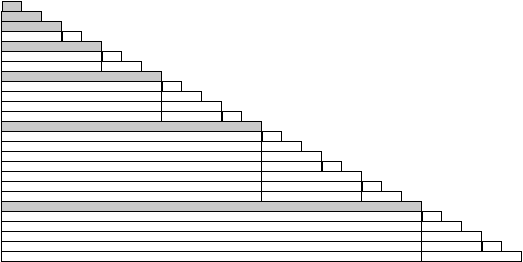
\includegraphics[scale=0.6]{FiguresArithmetic/Zeckendorf}
        \caption{The first integers (on the Y-axis) broken down into the Zeckendorf representation.
        The shaded rows corresponds to pure Fibonacci numbers.}
\label{zeckendorf}
\end{center}
\end{figure}

\noindent \textbf{Proof of Zeckendorf's Theorem}

The proof is done by induction on $n$ for proving simultaneously both construction and uniqueness.

\begin{itemize}
\item
The basis is true since the decomposition is obviously unique for $n=2$ (and also for $n=3$). 
Notice that for $n=4$, we have $4 = 3 + 1 = F(4) + F(2)$. 

\item
Assume for the induction step that any integer strictly lower than $F(k)$ can be decomposed uniquely as the sum of non-consecutive Fibonacci numbers.
We will prove as a consequence that an integer $n$ in the next interval between two consecutive Fibonacci numbers $F(k) \leq n < F(k+1)$ may be decomposed. 

If $n=F(k)$ is a Fibonacci number, the decomposition is reduced to $F(k)$.

Moreover, it is not difficult to check that it is unique.

%by using Property~\ref{prop:FiboSum}:
%$F(k) = 2+ \sum_{i=1}^{k-2} F(i)$ (the 2 comes from the shift of the starting element of the sequence...).

\medskip

If $n \neq F(k)$ write $n = F(k) + N$.

As $N$ is strictly lower than $F(k)$, we apply the recurrence hypothesis to decompose it into non-consecutive Fibonacci numbers:

$n = F(k) + F(k_1) + F(k_2) + \cdots + F(r)$ where $k_2 \gg ... \gg k_r \geq 2$. 

The last point to verify is that $F(k)$ and $F(k_1)$ are not consecutive ($F(k) \gg F(k_1)$), which is done by contradiction:

Assuming $k$ and $k_1$ are consecutive ($k_1=k-1$) leads to $n = F(k+1) + F(k_2) + \cdots + F(r)$
which contradicts $n < F(k+1)$.
\end{itemize}

Any unique system of representation is a numbering system.

The previous theorem ensures that any non-negative integer can be written
as a sequence of bits $b_i$, in other words,

$n = (b_mb_{m-1}...b_2)_F$ iff $n = \Sigma_{k=2}^m b_k F_k$.

Let us compare this system to the binary representation.
For instance, the Fibonacci representation of $12345$ is $(100001010000100000010)_F$
while  $12345 = 2^{13} + 2^{12} + 2^{5} + 2^{4} + 2^{3} + 2^{0} = (1100000111001)_2$.

The binary representation is more compact. 
\bigskip

The decomposition in the Fibonacci basis of the first integers (starting from $1 = (00001)_F$) is as follows:

 $2 = (0010)_2 = F_3 = (00010)_F$
 
 $3 = (0011)_2 = F_4 = (00100)_F$
  
 $4 = (100)_2 = 3+1 = (00101)_F$
 
 $5 = (101)_2 = F_5 = (01000)_F$
 
 $6 = (110)_2 = 5+1 = (01001)_F$
 
 $7 = (111)_2 = 5+2 = (01010)_F$
 
 $8 = (1000)_2 = F_6 = (10000)_F$
 
 $9 = (1001)_2 = (10001)_F$
 
 $10 = (1010)_2 = (10010)_F$
 
 $11 = (1011)_2 = (10100)_F$
 
 $12 = (1100)_2 = (10101)_F$
 
 $13 = (1101)_2 = F_7 =(100000)_F$
 
 ...
 
There is no consecutive digits equal to $1$ in such representations.
